%\documentclass[journal]{IEEEtran}
\documentclass{article}

\usepackage[textwidth=8.5in, textheight=11in, top=1.5in, bottom=1.5in, left=1in, right=1in]{geometry}

% correct bad hyphenation here
\hyphenation{op-tical net-works semi-conduc-tor}
% equalize two columns in the last page
\usepackage{flushend}

\usepackage{url}
%\usepackage[caption=false]{subfig}
\usepackage{subfigure}
\usepackage{array}
\usepackage{color}
\usepackage{booktabs}
\usepackage{multirow}
\usepackage{multicol}

\usepackage{algorithm}
\usepackage{algpseudocode}
\renewcommand{\algorithmicforall}{\textbf{for each}}
% \usepackage{setspace} % squeeze the vertical space in algorithm

% \makeatletter
% \renewcommand{\ALG@beginalgorithmic}{\small}
% \makeatother

\usepackage{amsmath}
% \usepackage{amsthm}
\usepackage{amssymb}
\usepackage{stmaryrd}


\newcommand{\squishlist}{
\begin{list}{$\bullet$}
{ \setlength{\itemsep}{0pt}
\setlength{\parsep}{3pt}
\setlength{\topsep}{3pt}
\setlength{\partopsep}{0pt}
\setlength{\leftmargin}{1.5em}
\setlength{\labelwidth}{1em}
\setlength{\labelsep}{0.5em} } }

\newcommand{\squishend}{  \end{list}  }

% shortcut
\usepackage{xspace}
\newcommand{\etc}{{etc.}\@\xspace}
\newcommand{\ie}{{i.e.,}\@\xspace}
\newcommand{\etal}{{et al.}\@\xspace}
\newcommand{\eg}{{e.g.,}\@\xspace}
\newcommand{\aka}{{aka}\@\xspace}

\newcommand{\termspace}{{\vspace{-0.15in}}}         
% control space after figure
%\newcommand\figsize{0.8\linewidth}
\newcommand\assize{1.3}
\newcommand\tablefontsize{\small}
\newtheorem{theorem}{Theorem}
\newtheorem{definition}{Definition}

\usepackage{graphicx}
\graphicspath{{figs/}}

\usepackage{indentfirst}
\usepackage{fixltx2e}
\newcommand{\wu}[1] {\textbf{\color{blue}{Wu: #1}}}
\newcommand{\tsub}[1]{\textsubscript{#1}}

\usepackage{multirow}
\newcolumntype{L}[1]{>{\raggedright\let\newline\\\arraybackslash\hspace{0pt}}m{#1}}
\newcolumntype{C}[1]{>{\centering\let\newline\\\arraybackslash\hspace{0pt}}m{#1}}
\newcolumntype{R}[1]{>{\raggedleft\let\newline\\\arraybackslash\hspace{0pt}}m{#1}}

\begin{document}

\title{Measurement of Crowdsourced Live Video on Server Side}

%\author{Jianer Zhou$^\dag$ $^\S$, Zhenyu Li$^\dag$, Qinghua Wu$^\dag$, Gaogang Xie$^\dag$ \\
%$^\dag$ICT-CAS, China,
%$^\S$Univ. of CAS, China\\
%\{zhoujianer, zyli, wuqinghua, xie\}@ict.ac.cn}
\author{}
\date{}
\maketitle

\begin{abstract}
As the popularity of intelligent medium device and improvement of bandwidth, more and more people are involved in the crowdsourced live video applications. Despite its great popularity, crowdsourced live video system in the wild has not been widely studied. This motivate us to analyze the the performance of a crowdsourced live video system in production network. In this work, we measure the effectiveness of this system through a packet-level trace collected from server side. We find that video upload process is the key of the overall performance as it influences the video download throughput and 37 \% of stalls in upload process cause stalls in download flows. Our findings provide new insights in such system and can help the designers to improve its effectiveness.
\end{abstract}

%!TEX root = main.tex

\section{Introduction}
\label{sec:introduction}

 As cell phones and intelligent medium devices have camera, people can use such devices to broadcast their own activities to the Internet and we call such video as crowdsourced live video. Now more and more people have involved in the such kind of video as the emergence of popular application, such as Google Glass, Twitch.tv, Intelligent monitor~\cite{ishimaru2014blink}. People make use of crowdsourced live video to monitor their houses, make social activities with other people and even advertise their business. 
 
 Traditional live video system can be divided into two types. One has stable providers and multiple viewers, such as YouTube and game broadcaster~\cite{Mukerjee2014CDNvideo} ~\cite{yin2009livesky}. In these live video systems, once the video is produced, it is delivered to CDN(Content Delivery Network) and viewers fetch the videos from the CDN. The other type has unstable provider and single viewer, such as FaceTime and Skype~\cite{Xu2012skype}. For viewer, such video is unstable as it can not be delivered to CDN first and has to go through WAN(Wide Area Network) entirely the path~\cite{Benson2010DCN}. However there are just single viewer and the video provider can deliver the video directly to the viewer. Crowdsourced live video is different from traditional live video as it has both unstable providers and multiple viewers.
 
 In crowdsourced live video system, anyone may post their video. System operators can not be sure which video will be popular and how long the video is, so it is unreasonable to deliver  the video to CDN. Viewers have to fetch the video from where it is produced which means the video is unstable for viewers. Multiple viewers mean that the providers can not make connections directly with viewers as the providers are often low power and low processing ability handheld devices. Such different features make the traditional system hard to meet the crowdsourced live video's needs. It is necessary to detail the architecture of such crowdsourced live systems and figure out how well they work.

There has been some work focused on the effectiveness and measurement for the crowdsourced video system. Simoens \etal~\cite{simoens2013sigasight} propose a system to storage and search the crowdsourced videos. However, the system does not focus on video broadcast process. Zhang \etal~\cite{zhang2015twitch} collect the traffic on client side to 'guess' the architecture of the crowdsourced video system and measure the user behaviour. Until now, there are not detail introduction to the crowdsourced live video system and the performance of such system has not been analysis in the wild. Motivated by this, in this paper we introduce the architecture of a crowdsourced live video system which has been deployed in the production environment and measure the effectiveness of this system by large packet-level traces collected in the front-end relay servers. In particular, our main observations are the following:

\newcommand{\squishlist}{
 \begin{list}{$\bullet$}
  { \setlength{\itemsep}{0pt}
     \setlength{\parsep}{3pt}
     \setlength{\topsep}{3pt}
     \setlength{\partopsep}{0pt}
     \setlength{\leftmargin}{1.5em}
     \setlength{\labelwidth}{1em}
     \setlength{\labelsep}{0.5em} } }

\newcommand{\squishend}{
  \end{list}  }

\squishlist
\item By using a front-end relay server, the crowdsourced live video can effectively upload and by caching the video temporarily on the front-end server the system can handle mulitple viewers scalable.

\item As the upload flows'  reorder rate grows, the flow rate drops greatly and viewers trend to stop uploading their video.

\item About 40\% of stalls on the upload process will cause the download flows do not have data to send and result in a stall in download flows.

\item In video flows, I frame(the most important frame in H.264) has the highest packet loss rate compared with P and V frames.
    
\squishend 

The rest of the paper is structured as follows. Section~\ref{sec:system} introduces the crowdsourced live video system and the overview of video frame. Section~\ref{sec:dataset} presents how we collect the dataset and the basic information of the datasets. In Section~\ref{sec:system-measurement} we measure the system's upload, download and their relationship in detail. Section~\ref{sec:frame-analysis} analysis the feature of different frames in H.264. Section~\ref{sec:summary} summarize the discovery we find and Section~\ref{sec:conclusion} concludes the paper. 
%!TEX root = main.tex

\section{System Overview and Dataset}
\label{sec:system}

%In this section, we begin with an overview of the architecture of the crowdsourced live video system, and next describe the dataset which we will investigate in the following sections.

%\subsection{Architecture of crowdsourced live video system}
%\label{sub:system-architecture}

Figure~\ref{fig:system} shows the architecture of the crowdsourced live video system, which consists of five components: a unique global controller, front-end servers, distributed storage system, video sharing users and video viewing users. As shown in the figure, global controller decides which front-end server to serve the video sharing or viewing requests. Aditya \etal ~\cite{ganjam2015c3} have proved that a controller can make video broadcast system effective.

Video frames generated by video sharing users are uploaded to storage system via the selected front-end server, using two TCP connections, in which connection 1 is from user to front-end server and connection 2 is from front-end server to storage system. Video viewing users request the desired video from storage system via the selected front-end server using connection 3 and 4. Note that the front-end servers are deployed in different locations and are scheduled according to the policy of the controller, thus the front-end server for sharing of a video may be different from those serving the viewing of that video. The flows amongst front-end servers and storage server traverse internal network with low latency and nearly zero packet loss. In contrast, the flows between front-end servers and users go through Wide Area Network (WAN) or cellar network, which has high packet loss rate and long latency. Thus in this work we mainly focus on analysis of the performance of flows between front-end servers and users.

%We use Cassandra cluster as our storage system. Cassandra is an key-value based open source distributed storage system which has been deployed in many large Internet company, such as Google, Facebook and Amazon~\cite{Beernaert2013cassandra}. It provide high availability and support clusters spanning multiple datacenters. 
\begin{figure}[ht]
	\centering
	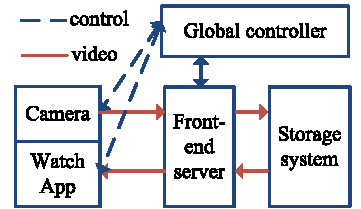
\includegraphics[width=2.5in]{system}
	\caption{An overview of the crowdsourced live video system.}
	\label{fig:system} 
	\termspace
\end{figure}

% \textbf{\textit{Post video:}} When consumers want to post a video, camera will first connect to the controller. The controller will select a best front-end server for it according the camera's location and network condition. Ganjam \etal~\cite{ganjam2015c3} find that a centralized control plane can improve the video quality in video broadcast platform. Cameras set up TCP connection 1 with the 'pick up' front-end server. The front-end server play two kinds of role: publisher and subscriber. Publishers receive the video from camera and the subscriber send video to viewers. After receiving the video from camera the publisher will set up TCP connection 2 to send the video to storage servers which is in the same DCN(Data Center Network) with the front-end servers. 

% \textbf{\textit{Watch video:}} When viewers want to watch a video, they also first connect to the controller. The controller will select the nearest front-end server which is also in the same ISP(Internet Service Provider) with consumer. Viewers set up TCP connection 3 with the 'pick up' front-end to request a live video. And then the front-end server will set up  TCP connection 4 to fetch the video from storage server. If the front-end server and video are in the same DCN, it will fetch the video directly. However, if the video is stored in other DCN, the front-end sever will fetch the video from remote DCN. Those DCNs in our system is connected directly by optical fiber which has a large bandwidth and short RTT. The front-end sever will cache the video temporarily that it is playing. When other consumers request the same video, the front-end servers will send back the video that is cached in it which make it unnecessary to fetch from storage servers. Such caching video solution makes our system scalable as even thousands of consumers request a same video, the front-end sever just needs to fetch the video only once.

% In totally, the crowdsourced live video system set up four TCP connections for a single live video watching process. The connections 2 and 4 are between front-end server and storage server and they both go through internal network which has low packet loss rate and short RTT. Connections 1 and 3: camera between front-end sever and front-end sever between viewers go through Wide Area Network (WAN) which has high packet loss rate and long RTT. In Section~\ref{sec:system-measurement} we will analyze the whole system based on the TCP connections, especially the influence caused by the two connections in unstable WAN.

%This is different from traditional live video system. When the traditional live video system broadcast a football game, the camera will transport the video to the front-end server and the front-end server will immediately deliver it to the CDN(Content Dilivery Network) both by stable internal network. As the video is delivered by stable internal netowrk, the traditional live video system has more stable video supply compared with crowdsourced live video system. And that also means that in traditional live video system the network factors that influence user experience is mainly on the connection between Apps and front-end server. However, in crowdsourced live video system the unstable connection between camera and front-end sever may also influence the system. 

% \subsection{Overview of video frame}
% \label{sub:video-frame}

H.264 is used as the video codec in the system, in which there are 4 types of frame: I, P, B and V~\cite{schwarz2007overview}. I frame is the key frame with largest size (10 - 100 Kbytes) and slowest production speed (0.25 f/s). P and B frames (both of which are called P frame for short in the following) are predicted frames with size 2 - 10 Kbytes. The production speed of P frame is 25 f/s and is adaptive according to the network quality. V frame carries voice data with size less than 1 Kbytes and production speed 25 f/s. 

% The video codec in our system is H.264 and we use RTMP(Real Time Messaging Protocol, which is based on TCP) ~\cite{zambelli2009iis} to transfer video. In H.264 there are four kinds of frame to produce a video: I frame, P frame, B frame and V frame. I frame is IDR(Instantaneous Decoder Refresh) frame, which is known as a keyframe and can build a without any other information ~\cite{timothy2011h264}.  P frame is Predicted frame which predicts the picture according the previous frame. B frame is Bidirectional predicted frame which predicts picture according the previous or future frame. In this paper, we do not distinguish P frame and B frame and call them both as P frame. V frame is the voice frame which records the voice along the video. The size and produced terminal of frame are different. I frame is often 10-100K bytes and is produced every 4 seconds. P frame is often 2-10K bytes and its produced terminal is unstable, changed according the dynamic of the video. The size of V frame is less than 1K bytes and our system produces 25 V frames every second. Different frames may have different performance in network. In Section~\ref{sec:frame-analysis} we will detail the different performance of each type of frame.


%For timeless storage and fetching the video, the storage unit in our Cassandra cluster is frame. Which means the system uses a key to storage and fetch echa frame.  

\iffalse
\begin{figure}[ht]
	\centering
	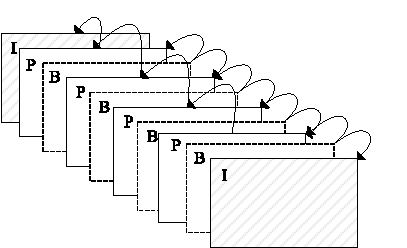
\includegraphics[width=2.5in]{frame}
	\caption{An overview of H.264 frame.}
	\label{fig:frame}
	\termspace
\end{figure}
\fi

The packet-level dataset we use for analysis was collected via tcpdump in one front-end server, which spans from Jul 15th, 2015 to Jul 22nd 2015. We captured all the video flows that go through the front-end servers. Overall, we collected 4.88 billion packets, corresponding to 1.24 million flows. The average packet size is 1028 bytes and average flow size is 3.86MB. Through examining the TCP ports that each packet is assigned, we could distinguish which one of the four connections (flows) the packet belongs. 
%%!TEX root = main.tex

\section{Datasets}
\label{sec:dataset}

\subsection{Data description}
\label{sub:data-des}
The four TCP connections of the front-end server use different port number to distinguish each other. We use tcpdump to collect the TCP traces of all the four connections in one front-end relay server. Our collection span from July 15, 2015 to July 22, 2015, totally 7 days, 24 hours each day. 

Figure~\ref{fig:use-fre} shows the users' upload and download times over one week. In the figure, we can observe that number of download flows is much higher than the number of upload flows, which means that more users watch video instead of sharing their videos. For both upload and download flows, they continue to grow after 6 a.m. and at about 11 p.m. they reach the peak. Consumers watch or share the crowdsourced live video more often in the night. And the peak of the whole week is at Saturday midnight. It is easy to understand as most people use the crowdsourced live video as a kind of entertainment and do not use it in work time. 

\begin{figure}[t]
\centering
\subfloat[Number of users' upload and download flows.]{
	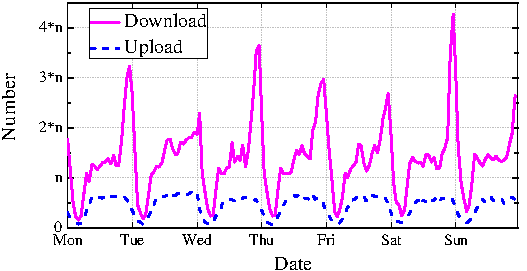
\includegraphics[width=2.5in]{use-fre}
	\label{fig:use-fre}}
\hspace{1em}%
\subfloat[Upload and download flows' complete time.]{
	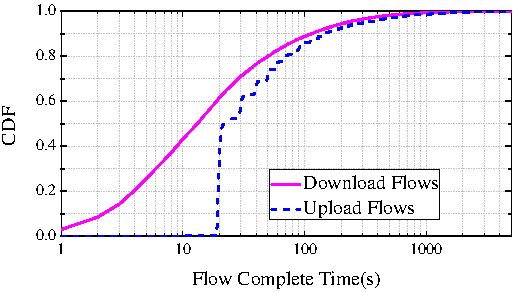
\includegraphics[width=2.5in]{flow-time}
	\label{fig:flow-time}}
	\hspace{1em}%
\subfloat[Upload and download flows' size.]{
	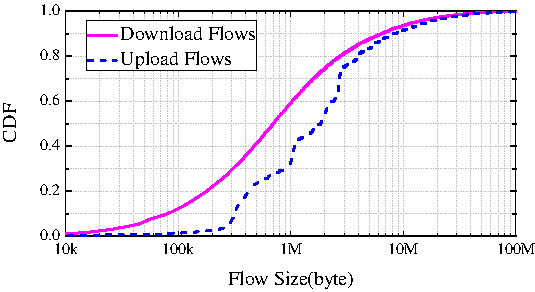
\includegraphics[width=2.5in]{flow-size}
	\label{fig:flow-size}}
\subfloat[The rate of upload and download flow.]{
	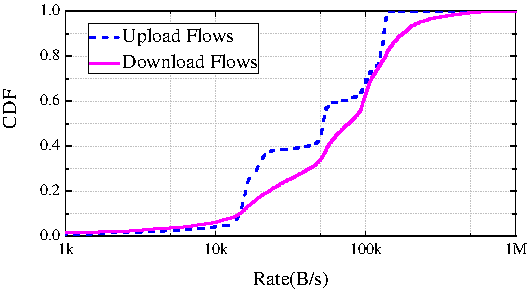
\includegraphics[width=2.5in]{rate}
	\label{fig:flow-rate}}
\caption{Dataset  description.}%
\label{fig:dataset} %% label for entire figure
\termspace
\end{figure}


\iffalse
\begin{figure}[ht]
	\centering
	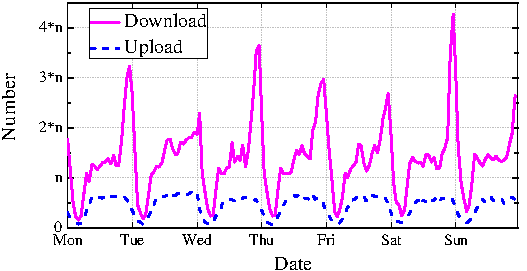
\includegraphics[width=\linewidth]{use-fre}
	\caption{Number of users' upload and download flows.}
	\label{fig:use-fre}
	\termspace
\end{figure}
\fi

Figure~\ref{fig:flow-time} shows the upload and download flows' flow complete time. For download flows, we define the flow complete time as the interval that the front-end server receives the first SYN packet until it receives the acknowledgment of the last packet. For upload flows, the flow complete time is defined as the interval that the front-end server receives the first SYN packet until it receives the last packet from the client. For upload flows, the servers will send keep-alive packet to keep the flow alive and will terminate the flows if it can not receive any frame from client until 20s. That is why there are almost not upload flows which are less than 20s. For both upload and download flows, about 60\% flows are less than 30s. That means most consumers watch or share short videos. As some viewers may terminate to watch the video while the video providers may continue to upload video, the flow complete time of upload flows are longer than download flows.   

%\begin{figure}[ht]
%	\centering
%	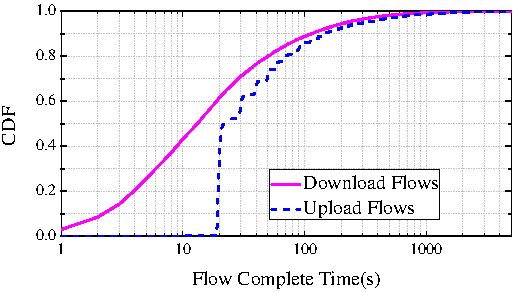
\includegraphics[width=\linewidth]{flow-time}
%	\caption{Upload and download flow complete time.}
%	\label{fig:flow-time}
%	\termspace
%\end{figure}

Figure~\ref{fig:flow-size} shows the upload and download flows' size. For upload and download flows, the flow size is defined as the whole packet size that the front-end severs receive or send. For download flows about 60\% flows are less than 1MB, and about 40\% upload flows are larger than 1MB, which means most of crowdsourced live videos are short. We can also see that download flows are smaller than upload flows, the same with the flow complete time.

%\begin{figure}[ht]
%	\centering
%	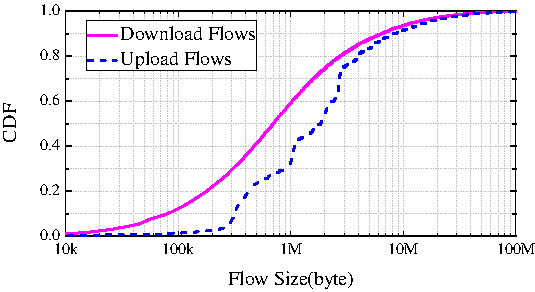
\includegraphics[width=\linewidth]{flow-size}
%	\caption{Upload and download flows size.}
%	\label{fig:flow-size}
%	\termspace
%\end{figure}

Figure~\ref{fig:flow-rate} shows the upload and download flows' rate. From the figure we can see that the upload flows' rate is smaller than the download flow. Two reasons account for it. First, for most network, the bandwidth of the upload is smaller than the download. For example, the upload bandwidth of ADSL(Asymetric Digital Subscriber Loop) is 640Kbps while the download bandwidth is 6-8Mbps~\cite{wei2008classification}. Second, as download flows is fetched from the storage server without waiting while the upload flows can only send data when cameras produce video data. 
%\begin{figure}[ht]
%	\centering
%	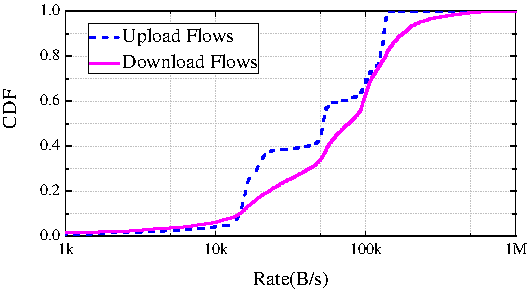
\includegraphics[width=\linewidth]{rate}
%	\caption{The rate of upload and download flow.}
%	\label{fig:flow-rate}
%	\termspace
%\end{figure}

%!TEX root = main.tex

\section{System Measurement}
\label{sec:system-measurement}

In this section, we use the TCP traces described above to measure our crowdsourced live video system. In Section~\ref{sub:upload-analysis} we will analyze the TCP upload flows, which transfer video data from camera to front-end server. In Section~\ref{sub:download-analysis} we will analyze the TCP download flows, which distribute video data from front-end server to viewers. And in Section~\ref{sub:relationship-analysis} we will analyze the relationship between the upload and download flows and try to figure out how the upload performance impacts the whole system performance.

\subsection{Analysis of TCP upload flows}
\label{sub:upload-analysis}

Video sharing users upload video to front-end server once they produce frames. The fluency of upload video directly impact the Quality of Experience of video viewing. Two factors may influence the upload process: one is the interval of frame producing process and the other is the delay by the network. We define \emph{TCP stall} as an event where the duration between two consecutive packets received/sent by the server is larger than $\min(\tau\cdot\text{SRTT}, \text{RTO})$. Parameter $\tau$ is set to 2 in this work as the TCP endpoint could at least receive or send one packet during $2RTT$ in the ideal condition. As the front-end server (where we collected the data) is the receiver in the upload flow, we can only measure the 3-Way HandShake (3WHS) RTT during which servers send a SYN packet and receive the corresponding acknowledgment. Thus, we use the RTT in 3WHS as the \text{SRTT} for this flow. 

The front-end server, as a receiver in the upload flow, may receive a series of disordered packets, in which the packets in the hole (\ie not received in sequential order) may be reordered by the network, or retransmitted because the previously transmitted segment is dropped. The front-end server could not distinguish whether the disordered packet is a packet reordering or packet retransmission. When a stall happens, receivers may have received a series of disordered packets, or sequential packets. We further distinguish the stalls by labeling the former as \emph{reordering stall} and the latter as \emph{normal stall}. When not receiving any video data from the camera, front-end server will send keep-alive packets, per in 5 seconds, to make the connection open. We find that all the stall time accounts for 31.6\% of all the completion time in the upload flows. Among these stalls, normal stall contributes 93.5\% of stall time, reordering stall contributes 1.3\% of stall time, keep-alive stall accounts for 5.2\% of stall time. It means that packet loss or reordering is not the main factor of network stalls. However, the interval of frame produced process is the main factor that influence the upload flow. That can also be confirmed by the fact that the median throughput of upload flows is 60KB/s, much smaller than the available upload bandwidth.

\iffalse
 The percentage of different stall time is shown in Table~\ref{tbl:upload-stall}.
\begin{table}[ht]
\tablefontsize
\renewcommand{\arraystretch}{\assize}
 \setlength{\tabcolsep}{3pt}
\caption{Percentage of different stall in upload flows.}
\centering
\begin{tabular}{c|c}
	\toprule
	 type & percentage(\%) \\
	\hline
	normal & 93.5 \\
	\hline
	reorder & 1.3 \\
	\hline
	keep alive & 5.2 \\
	\bottomrule
\end{tabular}
\label{tbl:upload-stall}
\termspace
\end{table} 
From Table~\ref{tbl:upload-stall}, we can see that 93.5\% stall is normal stall while the reorder stall is just 1.3\%. 
\fi

We define reordering rate as the ratio of packets which do not arrive in order to all data packets. We find that the overall reordering rate is about 1\% and among those disordered packets, 6\% of them suffer from timeout reordering, which means the interval between two disordered packets is larger than 0.2 second (\ie the minimum RTO set in Linux kernel). Although packet loss or reordering happens rarely, once it happens, it will significantly impact the performance of upload flows. We find that packet reordering strongly correlates with the size of upload flow, especially when the reordering rate becomes large. Table~\ref{tbl:reorder-rate-influence} shows the impact of reordering rate on upload flow size. When the reordering rate becomes larger, the performance of upload flows degrades dramatically.

% We further find that the total frame's reorder rate is 1\% and among the reorder packets 6\% suffer from timeout reorder. If the packet in upload flow is lost and can not be recovered by fast retransmit, the front-end server will receive a timeout reorder packet. We define the reorder packet as timeout reorder packet if the interval between the reorder packet and the last send-in data is larger than 0.2 second(the minimum RTO in linux kernel). Although packet loss or reordering is not the main factor that impacts the performance of upload flows, we find that packet reordering strongly correlates with the size of upload flow, especially when the reordering rate becomes large. Table~\ref{tbl:reorder-rate-influence} shows the impact of reordering rate on upload flow size. When the reordering rate becomes larger, the performance of upload flows degrades dramatically. 

% Although the packet loss or reorder is not the main factor that influences the upload flow rate, we find that packet reorder rate greatly influence the upload flow size, especially when the reorder rate becomes large. Table~\ref{tbl:reorder-rate-influence} shows the influence of reorder rate to upload flows. As reorder rate grows, the upload flows' flow rate, flow size and FCT(Flow Complete Time) become small. 

When the reordering rate is larger than 20\%, which means the network quality is very bad, the mean size of upload flows becomes 0.73MB, much smaller than the flow size (5.1MB) when the reordering rate is less than 10\%. The video sharing users also views the video that he or she uploads. If the upload network is bad and the reordering rate becomes high, video sharing user is likely to terminate the upload process. That is why the flow size suddenly drops when the reordering rate becomes large. 

\begin{table}[ht]
\tablefontsize
\renewcommand{\arraystretch}{\assize}
 \setlength{\tabcolsep}{3pt}
\caption{Impact of reordering rate on the performance of upload flows.}
\centering
\begin{tabular}{c|c|c|c}
	\toprule
	reordering rate & avg throughput & flow size & FCT \\
	\hline
	$<$10\% & 64KB/s & 5.1MB & 87.7s \\
	\hline
	10-20\% & 48KB/s & 4.7MB & 72.8s \\
	\hline
	$>$20\% & 17KB/s & 0.73MB & 60.7s \\
	\bottomrule
\end{tabular}
\label{tbl:reorder-rate-influence}
\termspace
\end{table}  

\subsection{Analysis of TCP download flows}
\label{sub:download-analysis}

To figure out what factors influence the download flows between front-end server and viewers, we analyze the stalls in the TCP download flow. The \emph{stall} in download flows is defined the same as in Section~\ref{sub:upload-analysis}. As the front-end server is the sender in the video viewing process, it could calculate RTT dynamically each time it receives acknowledgment of the transmitted data.

According to the position where each stall happens, we further classify these stalls into the following types. \emph{Timeout retrans} stalls are those caused by the timeout retransmissions. \emph{Resource constraint} stall happens when there is no data in the buffer to transmit and is often caused by that the camera does not upload data timely.%(the same as the normal stall in Section~\ref{sub:upload-analysis} \wu{Normal stall can also be triggered for other reasons, \eg zero receive window.}). 
\emph{Packet delay} stall is caused when the ACK packets are delayed, either by network or receiver. When a viewer does not have enough buffer to store the data it will reduce its receive window (rwnd) to zero, thus the front-end server can not send any data until the viewer enlarges its rwnd. Such a stall is defined as \emph{zero rwnd} stall. When there are no data to transmit, the front-end server will send a keep-alive packet every 5 seconds to prevent the connection to be terminated. Such a stall is labeled as \emph{keep alive} stall. In total the stall time occupies 35.2\% of the completion time of all download flows. Table~\ref{tbl:stall-download} shows the ratio of different stalls in terms of time in download flows.

\begin{table}[ht]
\tablefontsize
\renewcommand{\arraystretch}{\assize}
 \setlength{\tabcolsep}{3pt}
 \caption{Analysis for download flows}
 \centering
 \subtable[Ratio of different stalls in download flow.]{
\begin{tabular}{c|c}
	\toprule
	Stall Type & Percentage(\%)\\
	\hline
	resource constraint & 39.4   \\
	\hline
	packet delay & 8.2 \\
	\hline
	zero rwnd & 16.3 \\
	\hline
	keep alive & 10.1 \\
	\hline
	timeout retrans. & 22.8 \\
	\hline
	others & 1.5 \\
	\bottomrule
\end{tabular}
\label{tbl:stall-download}
}
\hspace{3em}
\subtable[Ratio of RTT over RTT\tsub{3WHS} when varying $in\_flight$.]{
\begin{tabular}{l|c}
	\toprule
	 $in\_flight$ & RTT/RTT\tsub{3WHS} \\
	\hline
	[0, 4KB) & 0.89 \\
	\hline
	[4KB, 8KB) & 1.08  \\
	\hline
	[8KB, 16KB) & 1.31  \\
	\hline
	[16KB, 32KB) & 1.38  \\
	\hline
	[32KB, 64KB) & 1.61 \\
	\hline
	[64KB, $\infty$) & 2.6  \\
	\bottomrule
\end{tabular}
\label{tbl:inflight-rtt}
}
\termspace
\label{tbl:download-flow-analysis}
\end{table}  

From Table~\ref{tbl:stall-download} we can see that the \emph{resource constraint} accounts for 39.4\% of all the download stall, the largest part amongst all, which is partially caused by the upload flows. In Section~\ref{sub:upload-analysis} we find that stalls account for 31.6\% of all upload flow time. As the camera stops sending data for a while, the front-end server does not have any data to send. About 16.3\% stalls belongs to \emph{zero rwnd} stall, which means the viewers' inability of receiving data will also greatly impact the performance of video viewing. \emph{Keep alive} stall accounts for 10.1\% of download stall time, indicating that there are users still waiting for some time to terminate the connection even when the video sharing user has stopped uploading video.
% \wu{Keep-alive stall is caused by that the data is unavailable for a long time (longer than 5 seconds), which does not mean the video upload flow has been terminated.}
22.8\% of stalls belong to \emph{timeout retrans}, which is caused by the network. In Section~\ref{sec:frame-analysis} we will further analyze the timeout retransmission stalls in detail.

\subsubsection{Analysis of RTT variation}
\label{sub:RTT}

RTT is an important factor that influences the flow rate. The flows with small RTT are more likely to get high flow rate. RTT is determined by two factors. One is the number of hops between two nodes which is controlled by the route algorithm. The other is the packets' cache time at the routers which is controlled both by the router buffer capacity and the volume of packets in the network. In the WAN, the route algorithm and router buffer capacity are out of the control of sever. The only way that the server can control the RTT is by controlling the packets that is sent to the network.

In table~\ref{tbl:inflight-rtt} we analyze the change of RTT when varying the $in\_flight$ size. Parameter $in\_flight$ represents the amount of data bytes sent already and not received yet by the viewers, which is defined as follows:
%\begin{footnotesize}
\begin{equation}
\label{eq:conserve}
\begin{aligned}
in\_flight = \enspace & packets\_out + retrans\_out \enspace - 
 (sacked\_out + lost\_out) \enspace ,
\end{aligned}
\end{equation}
%\end{footnotesize}
where $packets\_out$ is the data bytes between $snd\_una$ (the packet with highest sequence number the receiver has acknowledged) and $snd\_nxt$ (the next new byte the sender would transmit), $retrans\_out$ is the data bytes which is retransmitted but not yet acknowledged, $sacked\_out$ is the SACKed data bytes, and $lost\_out$ is the estimated dropped data bytes.

We examine the change of RTT by comparing it with the RTT calculated in the 3-way handshake (3WHS) phase (referred to as RTT\tsub{3WHS}). From table~\ref{tbl:inflight-rtt} we can see that as the $in\_flight$ becomes large, the RTT also becomes large. When the $in\_flight$ is 64KB, the RTT is even 2.6 times of the RTT\tsub{3WHS}. That means when there are large number of in flight packets, routers in the path need more time to process them and thus result in large RTT.

\iffalse
\begin{table}[ht]
\tablefontsize
\renewcommand{\arraystretch}{\assize}
\setlength{\tabcolsep}{3pt}
\caption{Ratio of RTT over RTT\tsub{3WHS} when varying $in\_flight$.}
\centering
\begin{tabular}{l|c}
	\toprule
	 $in\_flight$ & RTT/RTT\tsub{3WHS} \\
	\hline
	[0, 4KB) & 0.89 \\
	\hline
	[4KB, 8KB) & 1.08  \\
	\hline
	[8KB, 16KB) & 1.31  \\
	\hline
	[16KB, 32KB) & 1.38  \\
	\hline
	[32KB, 64KB) & 1.61 \\
	\hline
	[64KB, $\infty$) & 2.6  \\
	\bottomrule
\end{tabular}
\label{tbl:inflight-rdtt}
\termspace
\end{table}  
\fi


%\subsection{Storage TCP connection analysis}
%\label{sub:storage-analysis}
%In our live video system, when cameras upload video to front-end server it re-send it to the cassandra storage server to store the video. When the watch app request to view a video, the front-end server will fetch video from the cassandra storage server. For storage and fetching video on the cassandra, front-end server needs to setup two different TCP connections. At storage process, after front-end server send data to cassandra, cassandra will reply a message to the server to inform whether the data has been inserted successfully. At fetching process, front-end server send a key to cassandra, and then cassandra will reply data to front-end sever according the key. That means for both of storage and fetching connections, there are send-in and send-out data. In this section we will detail the  send-in and send-out data in both of two connections in detail. 

%\subsubsection{Storage process}
%\label{sub:storm}
%The send-out data in storage process is the data that need to store in cassandra, and the send-in data is the message to inform whether the data has been inserted successfully. Table~\ref{tbl:storage-data} shows the statistics in the storage process. From the table we can see that send-out data rate is small, just 35KB/s much smaller than the rate that the camera send data to front-end server. In our personal live video system, once the front-send server receives a image or voice frame from camera, it will storm the frame to cassandra. However when the front-end server sends out the frame to cassandra, it can not send next frame until it receives successful reply message from cassandra. 

%In DCN(Data Center Network) the packet loss rate is quite small, so the loss rate of send-out data is quite small, just 0.001\%. But surprisingly, we find that 69.8\% of the loss packets are recovered by timeout retransmission. After we analysis those timeout retransmission we find that all of them is caused by less pkt retransmission. As the front-end server can not send next frame until it receive the reply message, the packet in network often less than 3 packets(if the size of the frame is less than 3 packets). At such condition, the server can not receive enough dupacks to trigger fast retransmission.  

%As the send-in data just send reply message which is small and the time use to calculate the rate is the whole flow complete time, the rate of send-in is even samller than the send-out data, just 10KB/s. As the small packet loss rate and the one frame one reply charater of storage process, we can not find any reorder packets in send-in data.  
       
%\begin{table}[ht]
%\tablefontsize
%\renewcommand{\arraystretch}{\assize}
 %\setlength{\tabcolsep}{3pt}
%\caption{Send out and in analysis in storage process.}
%\centering
%\begin{tabular}{c|c|c|c}
%	\toprule
%	 type & rate & loss/reorder rate & timeout num/loss num \\
%	\hline
%	send-out & 35KB/s & 0.001\% & 69.8\% \\
%	\hline
%	send-in & 10KB/s & - & - \\
%	\bottomrule
%\end{tabular}
%\label{tbl:storage-data}
%\termspace
%\end{table} 

%\subsubsection{Fetching process}
%\label{sub:fetch}
%Once the watch-app send request to watch a live video, the front-end server begins to fetch data from cassandra. The cassandra store each image and voice frame individually, and each frame has an unique key. The front-end server fetch the frames of video one by one using their keys, and it will not fetch next frame util it successfully get a full frame. The send-out data in fetching data process is that the front-end server sends 'get data' message to cassandra, and the send-in data is that cassandra reply video frame to front-end server. Table~\ref{tbl:fetch-data} shows the statistics in the fetching process. From the table we can see that the rate in send-in data is 1.98MB/s, much larger than the rate of send-out in storming process. That is because the wathcing process is a little delay than the uploading data process of camera, which means the data has been stored in the cassandra. The reorder rate of the send-in data is also small, just 0.0124\%. And 33.2\% of the reorder packet is timeout retransmission data. We find that most of the timeout reorder packet is also less pkt retransmissio, similar with send-out data in storage process.

%Send-out data's rate is just 67KB/s, because the send-out data is small which just carries the request key. The loss rate is also small just 0.0125\%, but nearly all of the loss packets are recovered by timeout retransmission. That is because the send-out packets are the request packet carrying the key of the frame. Front-end server will not send out any data utill it receives the full frame. The loss packet can only recover by the timeout retransmission as there is only one packet in flight.  

%\begin{table}[ht]
%\tablefontsize
%\renewcommand{\arraystretch}{\assize}
% \setlength{\tabcolsep}{3pt}
%\caption{Send out and in analysis in fetch data process.}
%\centering
%\begin{tabular}{c|c|c|c}
%	\toprule
%	 type & rate & loss/reorder rate & timeout num/loss num \\
%	\hline
%	send-out & 67KB/s & 0.0125\% & 99.6\% \\
%	\hline
%	send-in & 1.98MB/s & 0.0124\% & 33.2\% \\
%	\bottomrule
%\end{tabular}
%\label{tbl:fetch-data}
%\termspace
%\end{table} 


\subsection{Relationship between TCP upload and download flows}
\label{sub:relationship-analysis}
In the above, we have investigated the TCP upload and download flows in our system separately. However, the upload flows may have impact on the performance of download flows if they are in the same session (\ie they are sharing and viewing the same live video). For example reordering in upload flows may cause the download flows have no data to transfer. In this section we will detail the relationship between these TCP upload and download flows.

The system assigns each live video a unique ID for sharing and viewing, so we can match the upload and download flows by the video ID. Our data is collected from one front-end server, thus not all flows could be matched due to that upload flow is from one server and download flows are from other servers. Figure~\ref{fig:up-down-rate} shows the throughput of upload and download flows respectively in the same session, each in a point. From the figure, we find that the most of the points spread along the $y = x$ line, which means that in most sessions the throughput of download flows is equal to that of the upload flow. This confirms that for the crowdsourced live video, the video upload process are the key of video viewing performance.

\begin{figure}[t]
\centering
\subfigure[Throughput of upload and download flows.]{
	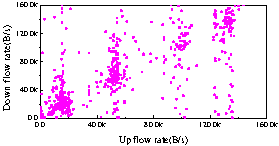
\includegraphics[width=1.8in]{up-down-rate}
	\label{fig:up-down-rate}}
\hspace{1em}%
\subfigure[FCT of upload and download flows.]{
	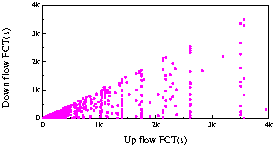
\includegraphics[width=1.8in]{up-down-fct}
	\label{fig:up-down-fct}}
	\hspace{1em}%
\subfigure[The corresponding download flow FCT with upload flow throughput.]{
	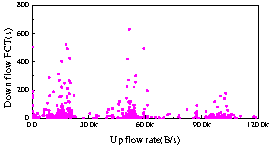
\includegraphics[width=1.8in]{up-rate-down-fct}
	\label{fig:up-rate-down-fct}}
\caption{Relationship between upload and download flows for the same video.}
\label{fig:relationship-up-down} %% label for entire figure
\termspace
\end{figure}


%\begin{figure}[ht]
%	\centering
%	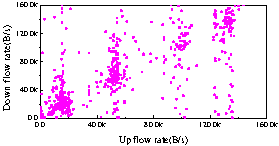
\includegraphics[width=\linewidth]{up-down-rate}
%	\caption{The corresponding rate of upload and download flows.}
%	\label{fig:up-down-rate}
%	\termspace
%\end{figure}

Figure~\ref{fig:up-down-fct} shows the FCT of upload and download follows. From the figure we can find that the points spread below the $y = x$ line, indicating that the FCT of download flows is shorter than that of upload flow. And we also find that the points spread discretely, which means that the FCT of download flows is independent with that of upload flows. Figure~\ref{fig:up-rate-down-fct} shows the relationship between the FCT of download flows and the throughput of upload flows. Most of the FCT of download flows is shorter than 200s. The throughput of upload flows is irrelevant with the FCT of download flows. Even when the throughput of upload flows grows to 100KB/s, most of the FCT of download flows is under 50s, nearly the same as when the throughput of upload flows is about 18KB/s. Figure~\ref{fig:up-down-fct} and Figure~\ref{fig:up-rate-down-fct} confirm that the FCT and throughput of upload flows do not have obvious influence on the FCT of the download flows. So we infer that the content features of the upload video are the key factor that impacts the FCT of download flows. 
%\begin{figure}[ht]
%	\centering
%	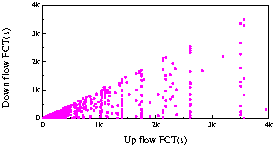
\includegraphics[width=\linewidth]{up-down-fct}
%	\caption{The corresponding flow complete time of upload and download flows.}
%	\label{fig:up-down-fct}
%	\termspace
%\end{figure}

%\begin{figure}[ht]
%	\centering
%	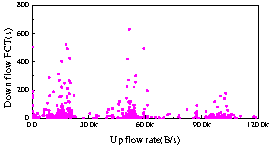
\includegraphics[width=\linewidth]{up-rate-down-fct}
%	\caption{The corresponding download flow FCT with upload flow rate.}
%	\label{fig:up-rate-down-fct}
%	\termspace
%\end{figure}

We also measure the impact of stalls in upload flows on the download flows. We find that 37.2\% of stalls in upload flows will cause stalls in download flows, most of which appear as \emph{resource constraint}, occupying the largest portion of the stalls in download flows. 
%Although we can not match the storage stall with download flows, we think most of the stall in storage flow will also cause \emph{resource constraint} stall in download flows. It is easy to understand as all the stall in upload and storage flows influence the data supply for download flows.
%!TEX root = main.tex

\section{Video frame analysis}
\label{sec:frame-analysis}

As mentioned in Section~\ref{sub:video-frame}, different frames in H.264 have different frame size and produced terminal and that will result in different network performance. In this section we will analysis in detail the different performance of I,P and V frame on the view of TCP connections. 

\subsection{Base video frame information}
\label{sub:base-frame}

Table~\ref{tbl:frame-info} shows the base information of different frames. Among all the three frames, P frame takes up 82.8 \%  of all the frames and is the largest part of all frames. The V frame has the smallest percentage of all frames just 5.8\% and the I frame is 11.5\%. In our system we set the I and V frame's produce interval as 4s and 0.04s respectively. We define the interval begins as the server sends out a frame until it sends out next frame. We find the actual intervals of I and V frames are 4.85s and 0.069s respectively because the change of RTT and packet loss may delay the frames. P frame does not have stable interval, different with the change of picture and its interval is 0.081s. I frame is the largest frame whose average size is 30K bytes. P frame's average size is 3.4K bytes while the V frame is just 189 bytes, much smaller than other two frames. The different frame size results in different burst packet number for different frames. V frame has no burst packet as its size is less than one packet size(most of the packet size is around 1460 bytes, same with MTU(Maximum Transmission Unit)). About 15\% P frame's burst packet number is larger than 5 packets, while for I frame about 40\% is larger than 5 packets. Routers has higher probability to drop burst packet, so the I frame's packet loss rate is 1.1\% which is higher than other two frames. P and I frame's packet loss rate is 0.6\% and 0.61\% respectively. Among these lost packets, some results in timeout retransmission, as they can not recover by fast retransmit. For I frame, 11.8\% loss packet result in timeout retransmission while for P frame and V frame it is 11.3\% and 14\% respectively. In Section~\ref{sub:timeout-frame} we will detail the timeout retransmission of different frames.

\begin{table}[ht]
\tablefontsize
\renewcommand{\arraystretch}{\assize}
 \setlength{\tabcolsep}{3pt}
\caption{Base information of different frame.}
\centering
\begin{tabular}{c|c|c|c|c|c}
	\toprule
	type  & per(\%) & interval(s) & size(B) &  loss rate(\%) &  timeout/loss(\%) \\
	\hline
	I   & 11.5 & 4.85 & 30K & 1.1  & 11.8 \\
	\hline
	P  & 82.8 & 0.081 & 3.4K  & 0.6 & 11.3 \\
	\hline
	V   & 5.8 & 0.069 & 189 & 0.61  & 14 \\
	\bottomrule
\end{tabular}
\label{tbl:frame-info}
\termspace
\end{table}  

\iffalse
\begin{figure}[ht]
	\centering
	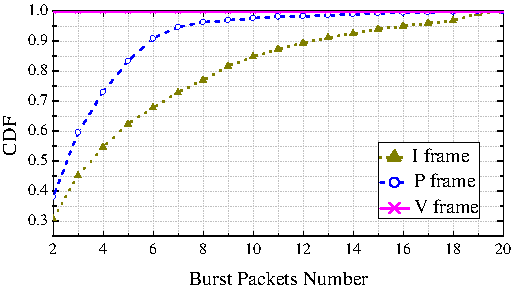
\includegraphics[width=\linewidth]{burst-frame}
	\caption{Different number of burst packets for different frames.}
	\label{fig:burst-frame}
	\termspace
\end{figure}
\fi

\subsection{Timeout retransmission of video frames}
\label{sub:timeout-frame}

If the fast retransmit can not recover a lost packet, it has to trigger timeout retransmission~\cite{flach2013reducing}. According the situation when the timeout retransmission happens, the timeout retransmission can be divided into several types. If the fast retransmit packet is drop by the network, timeout retransmission has to be triggered and we refer this timeout retransmission as double retrans. If the lost packet is the last three packets of the flow, there are not enough duplicate acknowledgments (dupacks) to trigger fast retransmit, we refer it as tail retransmission. Less dupacks to trigger fast retransmit may also because the server sends less than 4 packets out(either because there are not enough packets or the cwnd is small), and we refer it as less pkt retransmission. The ACK delay/loss or all of the packets send out lost will also result in timeout retransmission, as at both of the two situations no dupacks can be produced. We refer the two timeout retransmissions as  ACK delay/loss and continuous loss respectively. 

Table~\ref{tbl:time-out-frame} shows the time of each type of timeout retransmission for I, P and V frame. Those that cannot be classified into any of the above type of timeout retransmission is refered to as others. For all of the frames, the double retrans contributes the largest part of the timeout retransmission, 46.8\% for I frame, 44.7\% for P frame and 47.2\% for V frame. That is because when the network drops a packet, the network has high probability to become congested so the fast retransmit packet also has high probability to be dropped. For V frame, less pkt retransmission is 30.8\%, much higher than I and P frame which is 11.4\% and 20.2\% respectively. As the V frame is less than one MSS, when sending the V frame, there are often few packets in the network compared with sending I frame. That not only explains why less pkt retransmission is much higher for V frame, but also shed light on voice frame's high timeout retransmission rate in Table~\ref{tbl:frame-info}. In Table~\ref{tbl:frame-info} the V frame has smaller packet loss rate but higher timeout retransmission rate. The I and P frame has high burst packet number, the time that it is stored in the router is longer that V frame, so for I and P frames the ACK delay/loss timeout retransmission are 19.1\% and 15.1\%, much higher than V frame. Also because the different burst packet number, the continuous loss for V frame is 0, while 4.2\% and 1.5\% for I and P frame respectively.


\begin{table}[ht]
\tablefontsize
\renewcommand{\arraystretch}{\assize}
 \setlength{\tabcolsep}{3pt}
\caption{Timeout retransmission analysis for different frames.}
\centering
\begin{tabular}{c|c|c|c}
	\toprule
	 timeout retrans. type & I frame(\%) & P frame(\%) & V frame(\%)\\
	\hline
	tail retrans. & 3.8 & 4.0 & 5.0 \\
	\hline
	less pkt retrans. & 11.4 & 20.2 & 30.8 \\
	\hline
	double retrans. & 46.8 & 44.7 & 47.2 \\
	\hline
	ACK delay/loss & 19.1 & 15.1 & 8.5 \\
	\hline
	continuous loss & 4.2 & 1.5 & 0 \\
	\hline
	others & 14.7 & 14.4 & 8.5 \\
	\bottomrule
\end{tabular}
\label{tbl:time-out-frame}
\termspace
\end{table}  



%%!TEX root = main.tex

\section{Related work}
\label{sec:related}
%!TEX root = main.tex

\section{Findings and Implications}
\label{sec:summary}

\begin{table}
\tablefontsize
\renewcommand{\arraystretch}{\assize}
\setlength{\tabcolsep}{3pt}
\caption{Summary of findings and their implications.}
\centering
\begin{tabular}{L{3.2in}|L{3.2in}}
	\toprule
	\multicolumn{1}{c|}{Findings} & \multicolumn{1}{c}{Implications} \\
	\hline
	37\% of stalls in upload flows cause the download flows to have no data to transmit and thus result in a stall in download flows. & Optimizing of upload network and the performance of upload flows may greatly improve the performance of download flows. \\
	\hline
	When reordering rate in upload flow grows, the FCT of upload flows decreases greatly, which means the users tend to terminate video sharing if the network quality becomes bad. & Service provider could deploy front-end servers more nearer to video sharing users to optimize the upload performance, which may greatly improve the Quality of Experience (QoE) for both upload and download users. \\
	\hline
	Timeout retransmission contributes 29.8\% of stalls in download process. & Costly timeout retransmissions in short flows could be eliminated through slightly aggressively retransmission strategies, \eg \cite{flach2013reducing,zhou2015demystifying}. \\
	\hline
	Different types of frame experience different timeout retransmission characteristics due to their distinct frame production speeds and frame sizes, \eg I frame experiences more \emph{continuous loss} stalls while V frame experiences more \emph{less pkt retrans} stalls. & Transmit each type of frame in separate connections, and optimize each connection by eliminating the timeout retransmissions according to the characteristics of frames and connections. \\
	\bottomrule
\end{tabular}
\label{tbl:summary}
\termspace
\end{table}

Table~\ref{tbl:summary} summarizes the main findings and implications of our measurement results. Overall, our major findings could be grouped into two categories, one is the significant impact of upload performance on the involvement of view sharing and on the Quality of Experience of video viewing, the other is the distinct distribution of timeout retransmission stalls in different types of frame.

As the upload performance is vital to the overall performance of the crowdsourced live video system, more front-end servers should be deployed in different locations and the nearest one with better network quality (\ie lower delay and lower packet loss rate) should be selected for the video sharing users, to gain a better upload performance.

Even through previous work \cite{flach2013reducing,zhou2015demystifying} found the great degradation of performance of short flows due to timeout retransmission, we in this paper further find that flows may exhibit distinct characteristic of timeout retransmission due to different frame production intervals and frame sizes. To eliminate these costly timeout retransmissions, one could adopt existing solutions like TLP~\cite{flach2013reducing}, S-RTO~\cite{zhou2015demystifying}. Service provider could also optimize the performance by transmitting different frames in separate connections. Since the drop of a P or V frame can only hurt the watching experience slightly, P and V frames could be delivered in UDP connections and I frame is transmitted in TCP connection. Divide-and-conquer optimization of each type of connection may bring more performance improvement of the overall system.
%!TEX root = main.tex

\section{conclusion}
\label{sec:conclusion}
 
We present the architecture of a crowdsourced live video system in practice and analyze the effectiveness of the system by packet-level TCP traces. Video upload process is key as it significantly impact the throughput of video download flows and 37 \% of stalls in upload flows trigger stalls in download flows. Different frames have different performance in video flows. These finding may shed light on how to construct a high-performance crowdsourced live video system. 

\bibliographystyle{abbrv}
% \small
\bibliography{reference}

\end{document}
